\begin{figure}[!t]
    \begin{minipage}[!t]{0.48\textwidth}
        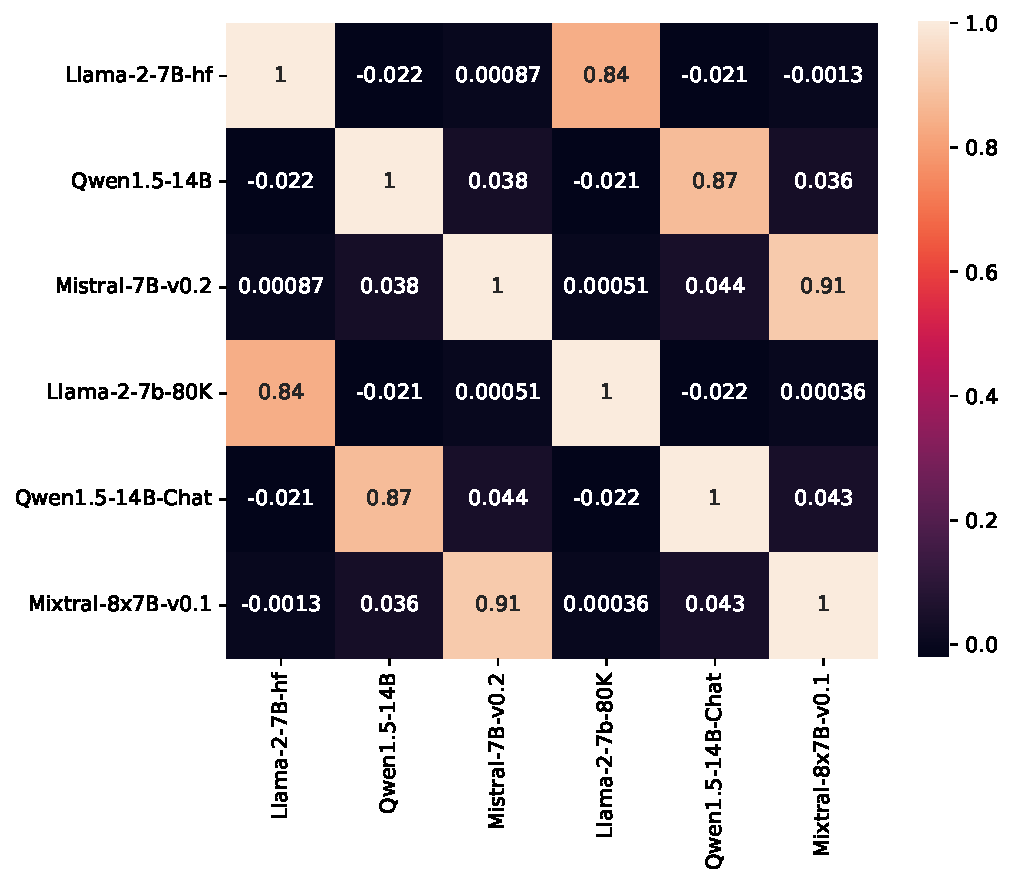
\includegraphics[width=\textwidth]{figures/corr_map.pdf}
        \caption{The retrieval heads of models of the same family are strongly correlated, i.e., the chat model and base model typically uses the same set of retrieval heads.
        The retrieval heads of models of different families are clearly different. 
        % For models of different families, their retrieval heads are clearly different. 
        }
        \label{fig:corr_map}
    \end{minipage}
    \hfill
    \begin{minipage}[t!]{0.48\textwidth}
        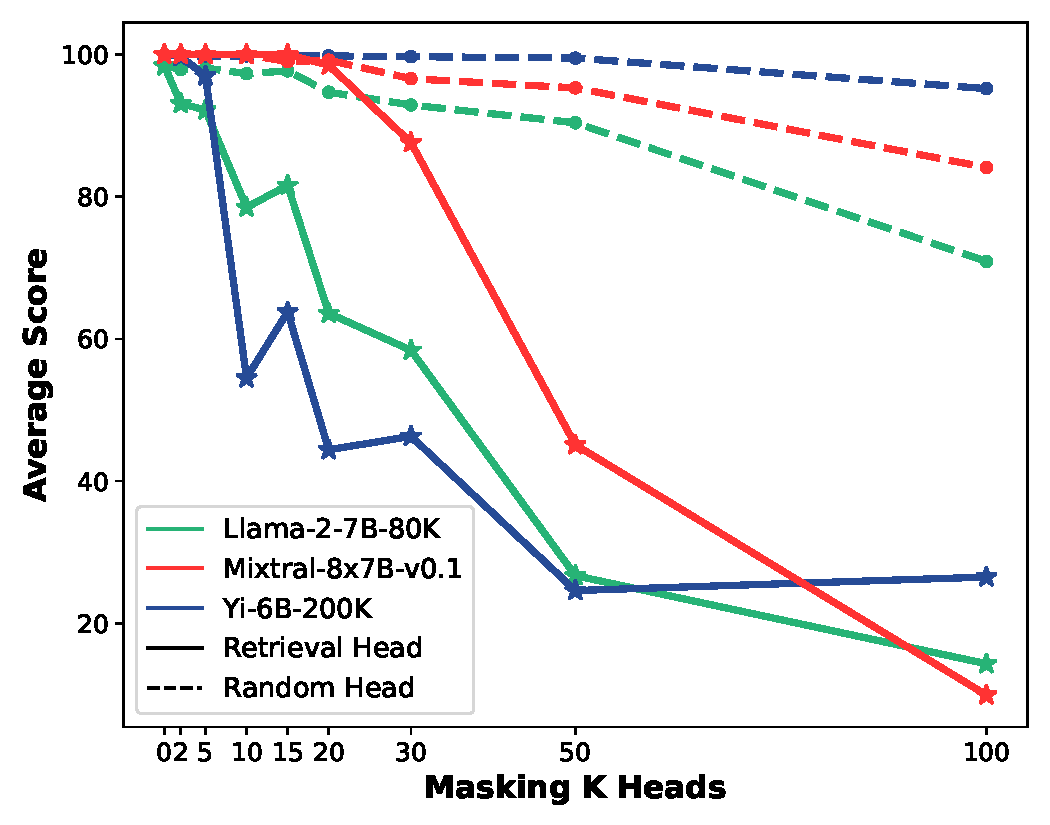
\includegraphics[width=\textwidth]{figures/masking_heads.pdf}
        \caption{Masking out top K retrieval heads vs K random heads. For all models are consider, the removal of retrieval heads clearly reduces the Needle-in-a-Haystack performance, versus the removal of non-retrieval heads have much weaker influence. 
        }
        \label{fig:needle_mask}
    \end{minipage}
\end{figure}
